% ------------------------------------------------------------------
% StepCheck -- ICSOC 2026 -- Introduction, revised
% Changes vs. intro__2_.tex:
%  (a) Para 3: "paths are syntactic" -> "path expressions are
%      syntactically valid" (clearer English).
%  (b) Para 4: removed the internal redundancy (native facts were
%      characterized twice); "unifying contribution" ->
%      "architectural contribution" to set up the hierarchy.
%  (c) Para 5: "Around it" -> "Within this architecture ... over the
%      same IR", resolving the two-competing-centres problem: the IR
%      is the framework, the shape analysis is the core technical
%      result inside it.
%  (d) Contributions bullet 4: "100% recall" -> "616/616 ... exact
%      per-class CIs" (consistent with the no-bare-100% policy of
%      Sect. 5); adds deployment-artifact corpora, three user-reported
%      faults, the three-verifier comparison, and industrial/case-study
%      highlights.
%  (e) Citation order in para 3 rearranged so the rendered numbers
%      appear ascending with the current .bib numbering; re-check at
%      camera-ready if the bibliography changes.
% ------------------------------------------------------------------

\section{Introduction}
\label{sec:intro}

Serverless applications increasingly encode business processes as managed workflows. In AWS Step
Functions, the executable artifact is an Amazon States Language (\asl) state machine: JSON for task
calls, branches, retries, parallelism, and error handling~\cite{awsStepFunctions}. These workflows
charge cards, reserve inventory, move documents, and coordinate human approvals, so latent workflow
bugs become production failures rather than local exceptions.
Figure~\ref{fig:intro} shows one such workflow. It passes AWS's syntactic validation, yet five latent defect classes survive and a sixth is one
edge away. \textbf{(1)} \code{ChargeCard} reads a missing \texttt{\$.total};
\textbf{(2)} reordering a single edge would let it ship before payment; and \textbf{(3)} a broad
retry can double-charge. The same workflow also shows \textbf{(4)} two parallel branches updating
the same item, \textbf{(5)} a callback that can wait forever, and \textbf{(6)} a committed
reservation without compensation.
Existing validators check that the JSON is well-formed, transitions exist, and path expressions are
syntactically valid~\cite{awsValidateDefinition,awsStatelint,aslValidator}. They do not check whether
a task produces the field its successor reads, whether a retry is safe for a non-idempotent effect,
whether two branches race on one resource, or whether a durable effect is compensated after
failure. The missing facts are semantic: task contracts, protocol states, idempotency, write
footprints, time bounds, and compensators. Formal workflow-soundness verifiers reason about
control-flow structure, not \asl{}'s data movement, retry, or compensation semantics, and flag valid
multi-terminal serverless workflows as unsound~\cite{woflan,bpmnanalyzer,bprove}. Durable-execution
systems enforce recovery at run time~\cite{burckhardt2021durable}, not before deployment.

\begin{figure}[t]
\centering
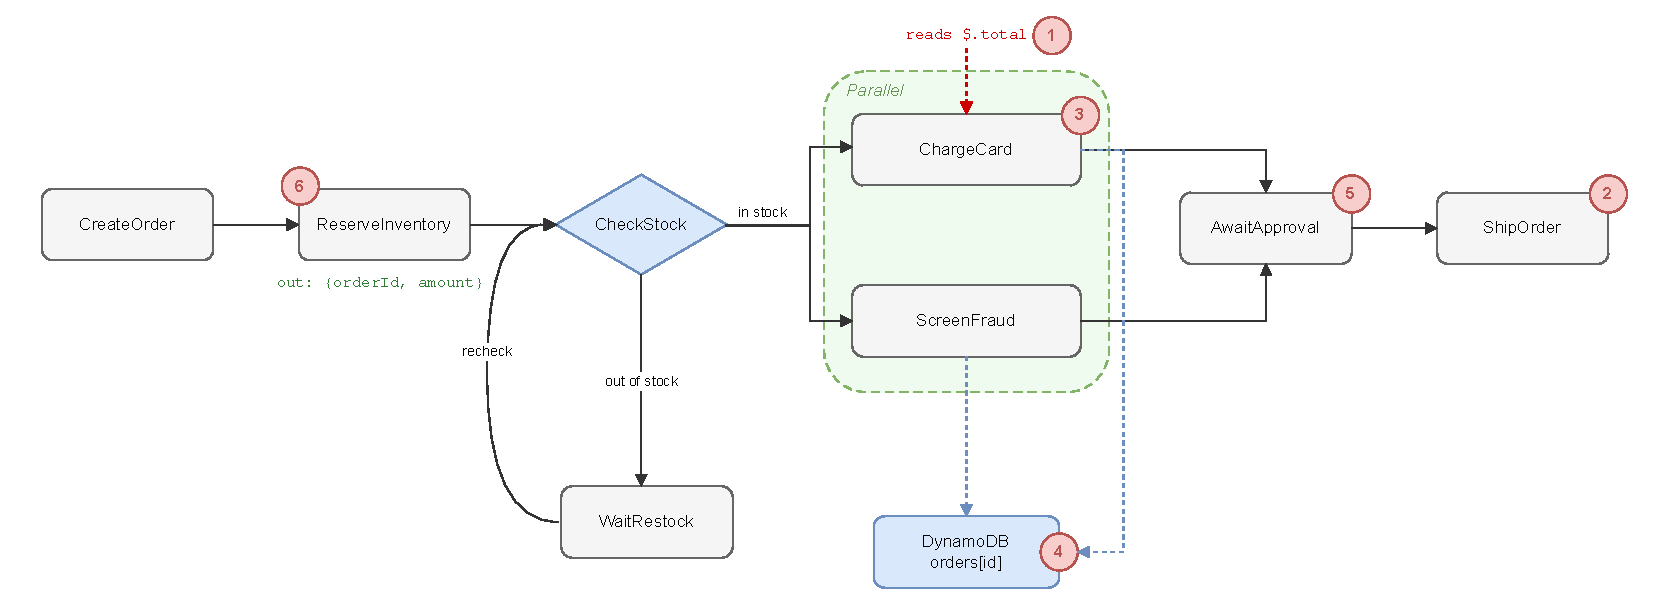
\includegraphics[width=1\linewidth, height=4.5cm]{figures/figure1-workflow.pdf}
\caption{An order-processing workflow that passes AWS's syntactic validation yet hides five latent defect classes, with a sixth one edge away; marker \textbf{(2)} is a one-edge ship-before-pay mutation, not an existing edge.}
\label{fig:intro}
\end{figure}


We present \tool{}, a static verifier for AWS Step Functions. Its thesis is simple: verify the
\emph{deployed artifact} under \emph{layered semantics}. The architectural contribution is a single
workflow IR with a \emph{provenance-aware} guarantee model. Facts native to \asl{} support
immediate structural, data-flow, temporal, and concurrency checks that are either sound---every error
report a true positive under the modeled semantics (Theorem~\ref{thm:soundness})---or deliberately under-approximating. The business facts
\asl{} omits---contracts, protocol states,
idempotency, persistence, compensators---are recovered as provenance-labelled premises from a
sidecar, typed DSL, generated metadata, or lightweight inference, and \tool{} grades every finding
by that provenance: inferred facts produce warnings, declared facts produce errors relative to the
declared model, so a finding's severity encodes the strength of the evidence behind it. Adoption
therefore starts on raw \asl{} and strengthens as teams add semantics.
Within this architecture, the core technical result is a flow-sensitive JSON-shape analysis for
\asl{}'s I/O pipeline: it reports a missing-field access \emph{as an error} only when, under the modeled semantics,  every execution reaching the
read lacks the field (Theorem~\ref{thm:soundness}). Seven further passes over the same IR cover
structural correctness, typed contracts, typestate ordering, retry safety, Saga compensation,
conservative concurrency, and temporal bounds.
In evaluation, \tool{} surfaces genuine, deployable defects in real workflows---an industrial
automotive case study whose lead developer confirmed timeout, data-flow, and concurrency faults,
faults re-discovered in production fix-commit and issue-tracker reports, and findings across
independent public repositories---and runs as a drop-in build-time gate (below 21\,ms) that blocks
semantic defects the deployed AWS validator accepts. Our contributions are:

\begin{itemize}
  \setlength{\itemsep}{1pt}
  \item A deployed-artifact verification architecture for \asl{} with native and declared semantic layers.
\item A data-flow analysis for missing JSON fields whose
error-level reports are free of false positives under the
modeled JSONPath/JSONata semantics, plus workflow checks for
retry, ordering, concurrency, time, and compensation. 
  \item A Rust implementation with raw \asl{}, typed-DSL, CNCF Serverless Workflow, and CloudFormation/SAM/CDK front ends.
  \item Empirical evidence that these defect classes occur in deployed
workflows and evade both industrial validators and formal soundness
verifiers---whose single-sink soundness conversely misclassifies
8--29\% of valid multi-terminal workflows---via mutation studies, a
developer-confirmed industrial case study, re-found production faults,
cross-format artifacts, and a sub-21\,ms CI gate.
\end{itemize}
